\documentclass[12pt]{article}
\usepackage{amsmath, amssymb, amsthm, epsfig}
\usepackage{listings}
\usepackage{fontspec}
\setmonofont{DejaVu Sans Mono}
\usepackage{tikz}
\usetikzlibrary{math,decorations.pathreplacing, shapes.geometric}
\usepackage{quiver}
\usepackage{float}
\usepackage{subcaption}

\usepackage[T1]{fontenc}
\usepackage[utf8]{inputenc}
\usepackage[fixed]{fontawesome5}
\usepackage{pifont}
\usepackage{bbding}

\theoremstyle{definition}
\usepackage{enumitem}
\newenvironment{Proof}{\noindent {\sc Proof.}}{$\Box$ \vspace{2 ex}}
\newenvironment{Solution}{\noindent {\sc Solution.}}{$\Box$ \vspace{2 ex}}


\usepackage{color}
\definecolor{keywordcolor}{rgb}{0.7, 0.1, 0.1}   % red
\definecolor{tacticcolor}{rgb}{0.0, 0.1, 0.6}    % blue
\definecolor{commentcolor}{rgb}{0.4, 0.4, 0.4}   % grey
\definecolor{symbolcolor}{rgb}{0.0, 0.1, 0.6}    % blue
\definecolor{sortcolor}{rgb}{0.1, 0.5, 0.1}      % green
\definecolor{attributecolor}{rgb}{0.7, 0.1, 0.1} % red

\def\lstlanguagefiles{../lstlean.tex}

\oddsidemargin-1mm
\evensidemargin-0mm
\textwidth6.5in
\topmargin-15mm
\textheight8.75in
\footskip27pt

\usepackage[table]{xcolor}
\definecolor{truecolor}{RGB}{198,239,206} % Light green
\definecolor{falsecolor}{RGB}{255,199,206} % Light red
\newcommand{\true}{\cellcolor{truecolor}T}
\newcommand{\false}{\cellcolor{falsecolor}F}
\begin{document}

\noindent \textit{\textbf{Math 300, Winter 2026}} \hspace{1.3cm} \textit{\textbf{HOMEWORK 2}} \hspace{1.3cm} 
\textit{\textbf{Grant Yang}
} 


\vspace{0.5cm}

\begin{Solution}
{\bf (\S2.1, Problem 6)}\\
No, $\{a,b,c\} = \{a,b,d\}$ does not imply that $c = d$. Consider the counter-example $c = a$ and $d = b$ with $a \ne b$. Then $\{a,b,c\} = \{a,b,d\}=\{a,b\}$, but $c \ne d$.
\end{Solution}


\vspace{0.5cm}

\begin{Solution}
{\bf (\S2.3, Problem 2)}\\
Let $A=\{1,2,\pi\}$ and let $P(x)$ be the statement $x\in\mathbb{Z}\land x\in A$. Then:
\begin{enumerate}[label=\alph*.]
\item $[\exists (x \in \mathbb{R}), P(x)] \implies \forall (x \in \mathbb{R}), P(x)$ is False. The left-hand side of the implication is True as the existential quantifier is satisfied by $x=1$, which satisfies $P(x)$. However $x=\sqrt{2}$ does not satisfy $P(x)$, so the for-all quantifier fails, and we have $\text{True}\implies\text{False}$, which is False.
\item $[\forall(x\in\mathbb{R}),P(x)]\implies \exists(x\in \mathbb{R}),P(x)$ is True. The left-hand side of the implication is False, as we can show that the counter example $x=\sqrt{2}$ does not satisfy $P(x)$. Because the hypothesis of our implication is not satisfied, the statement form as a whole evaluates to True.
\end{enumerate}
\end{Solution} 


\vspace{1cm}

\begin{Solution}
{\bf (\S2.3, Problem 9)}\\
Considering an underlying universal set of $\mathbb{R}$, 
\begin{enumerate}[label=\alph*.]
\item $(x\ge 0) \implies \exists y, y^2 = x$ is True: square roots of non-negative real numbers exist.
\item $(x\ge 0) \implies \exists!y,y^2=x$ is False: we can have $y=\pm \sqrt{x}$ (not unique).
\item $\forall x, \exists!y, y^3 = x$ is True: there is exactly 1 real cube root. ($x \mapsto x^3$ is a bijection $\mathbb{R}\to \mathbb{R}$)
\item $\exists!x, \forall y, xy=y$ is True: $x=1$.
\item $\forall x, \exists!y, xy=0$ is False: for $x=0$, there is no unique choice of $y$.
\item $\exists x, \exists!y,xy=0$ is True: choose any $x\ne 0$, and $y$ is uniquely determined to be $y=0$ as there are no nonzero zero divisors in $\mathbb{R}$.
\item $\forall x, \exists! y, x+y=0$ is True: $y=-x$ is the unique solution.
\item $\lnot\exists x,\forall y, x \le y$ is True: $y=x-1$ is a counterexample to the inner statement of the negation, meaning the expression as a whole is True. $\mathbb{R}$ is unbounded.
\end{enumerate}
\end{Solution} 


\vspace{1cm}
\newpage{}
\begin{Solution}
{\bf (\S2.4, Problem 4)}\\
\begin{enumerate}[label=\alph*.]
\item $A \subset B \implies B \not\subset A$. For contradiction, assume that $B \subset A$. Then we have $A \subset B\land B\subset A$, and after expanding the definition of strict subset, we get $(A \subseteq B \land A\ne B) \land (B \subseteq A\land B \ne A)$. Simplifying, this becomes $(A\subseteq B\land B\subseteq A)\land A\ne B$. However, by the theorem on set equality, $A \subseteq B \land B\subseteq A\iff A =B$, we have $A = B\land A \ne B$, which is a contradiction. Thus, our assumption must have been false, and $B \not\subset A$.
\item $A \subseteq \varnothing \implies A =\varnothing$. For all sets $A$, we can show $\varnothing \subseteq A$ since $\forall x, (x \in \varnothing \implies x\in A)$ is trivially true as there do not exist any $x \in \varnothing$. Thus, we have both $A \subseteq \varnothing$ and $\varnothing \subseteq A$, so by the theorem on set equality, we have $\forall x, (x \in \varnothing \iff x \in A)$ and thus $A = \varnothing$.
\end{enumerate}
\end{Solution} 


\vspace{1cm}

\begin{Solution}
{\bf (\S2.4, Problem 8)}\\
Let $A$ and $B$ be sets. We show that $A \subseteq B$ if and only if $\forall (U \in \mathcal{P}(A)), U\subseteq B$. Consider the backward direction of implication ($\forall(\dots) \implies A \subseteq B$). By the definition of subset, $A \subseteq A$ since $\forall x, (x\in A \implies x\in A)$ is trivially true. Since $A \in \mathcal{P}(A)$, we can apply the hypothesis (since $A$ satisfies our $\forall$) to obtain $A \subseteq B$. Now consider the forward direction, and let $U \subseteq A$ be a subset of $A$. Since $U \subseteq A \subseteq B$, we have $U \subseteq B$: for all $x \in U$, we derive that $x \in A$ using $U \subseteq A$, and we derive that $x \in B$ from $A \subseteq B$.
\end{Solution} 


\vspace{1cm}

\begin{Solution}
{\bf (\S2.4, Problem 10)}\\
It is false that $\{\{\{5\}\}\}=\{\{5\}\}$. By the definition of set equality, this means that $\forall x, (x \in \{\{5\}\}\iff x\in\{\{\{5\}\}\})$. However, $x=\{5\}$ is a direct counterexample to this: $\{5\} \in \{\{5\}\}$, but $\{5\}\not\in\{\{\{5\}\}\}$.
\end{Solution} 


\vspace{1cm}
\newpage{}
\begin{Solution}
{\bf (\S2.5, Problem 6)}\\

\begin{figure}[H]
    \centering
    % --- FIRST SUBFIGURE ---
    \begin{subfigure}[b]{0.48\textwidth}
        \centering
        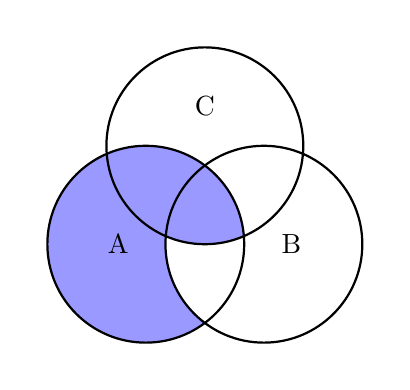
\begin{tikzpicture}[scale=0.5]
            % Fixed Bounding Box for alignment
            \useasboundingbox (-4.5,-3) rectangle (4.5,5.5);

            \def\circleA{(-1.5,0) circle (2.5)}
            \def\circleB{(1.5,0) circle (2.5)}
            \def\circleC{(0,2.5) circle (2.5)}
            \def\boundingbox{(-5,-5) rectangle (5,5)}
            
            % Shading logic: A \ (B \ C)
            \fill[blue, opacity=0.4] \circleA;
            \begin{scope}[even odd rule]
                \clip \circleA;
                \clip \circleB;
                \clip \circleC \boundingbox;
                \fill[white] \boundingbox; 
            \end{scope}

            % Outlines and Labels
            \draw[thick] \circleA;
            \draw[thick] \circleB;
            \draw[thick] \circleC;
            \node at (-2.2,0) {A};
            \node at (2.2,0) {B};
            \node at (0,3.5) {C};
        \end{tikzpicture}
        \caption{Region: $A \setminus (B \setminus C)$}
        \label{fig:venn1}
    \end{subfigure}
    \hfill
    % --- SECOND SUBFIGURE ---
    \begin{subfigure}[b]{0.48\textwidth}
        \centering
        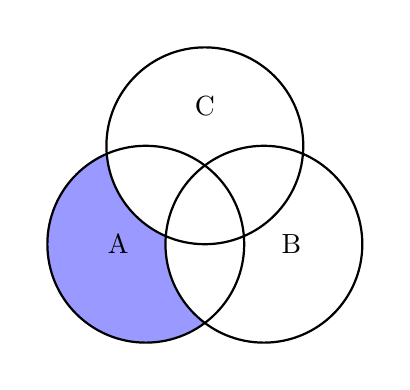
\begin{tikzpicture}[scale=0.5]
            % Same Bounding Box
            \useasboundingbox (-4.5,-3) rectangle (4.5,5.5);

            \def\circleA{(-1.5,0) circle (2.5)}
            \def\circleB{(1.5,0) circle (2.5)}
            \def\circleC{(0,2.5) circle (2.5)}
            \def\boundingbox{(-5,-5) rectangle (5,5)}

            % Shading logic: (A \ B) \ C
            \begin{scope}[even odd rule]
                \clip \circleB \boundingbox;         
                \clip \circleC \boundingbox;
                \fill[blue, opacity=0.4] \circleA; 
            \end{scope}

            % Outlines and Labels
            \draw[thick] \circleA;
            \draw[thick] \circleB;
            \draw[thick] \circleC;
            \node at (-2.2,0) {A};
            \node at (2.2,0) {B};
            \node at (0,3.5) {C};
        \end{tikzpicture}
        \caption{Region: $(A \setminus B) \setminus C$}
        \label{fig:venn2}
    \end{subfigure}
\end{figure}

Counterexample to the proposition that $A \setminus (B \setminus C)=(A\setminus B)\setminus C$: consider $A=\{1,2\}$, $B=\varnothing$, and $C=\{1\}$. Then $B \setminus C=\varnothing$, and $A\setminus B=A$. Thus, $A\setminus(B\setminus C)=A\setminus\varnothing=A$, but $(A\setminus B) \setminus C = A\setminus C = \{2\}$. Thus, $A \setminus (B \setminus C)\ne(A\setminus B)\setminus C$.
\end{Solution} 


\vspace{0.2cm}

\begin{Solution}
{\bf (\S2.5, Problem 10)}\\
Define the symmetric difference $A \oplus B:= (A\setminus B)\cup (B\setminus A)$.
\begin{enumerate}[label=\alph*.]
\item $A \oplus A=(A \setminus A)\cup (A\setminus A) = \varnothing \cup \varnothing =\varnothing$.
\item $A \oplus \varnothing = (A\setminus \varnothing)\cup (\varnothing \setminus A)=A\cup \varnothing = A$.
\item We have that $\forall (A,B,C), (A\cup B) \setminus C=(A\setminus C) \cup (B \setminus C)$ (proof by definitions, as $x \in (A\cup B)\setminus C$ and $x \in (A \setminus C) \cup (B\setminus C)$ both amount to ($x \in A$ or $x \in B$) and $x \not \in C$ as logical and distributes over logical or). \begin{align*}
    (A \oplus B)\setminus (A\setminus B) &= [(A \setminus B)\cup (B\setminus A)]\setminus (A\setminus B) \\
    &= [(A\setminus B)\setminus(A\setminus B)]\cup [(B\setminus A)\setminus(A\setminus B)] \\
    &= \varnothing \cup [(B\setminus A)\setminus (A\setminus B)] \\ &= (B\setminus A)\setminus (A\setminus B)
    =  \boxed{B\setminus A}.
\end{align*}
We have that $(B \setminus A) \setminus (A \setminus B) = B\setminus A$ since for all $x \in B \setminus A$, we have by the definition of set difference that $x \not \in A$. Thus, $x \not \in A\setminus B$, so doing the top-level set difference does nothing to $B \setminus A$.
\item Proving $A\oplus B=\varnothing \implies A = B$. Unfolding the definition of symmetric difference, we have that $(A \setminus B)\cup (B \setminus A) = \varnothing$. This implies that $A \setminus B =B\setminus A=\varnothing$, as if there existed an element $a \in A \setminus B$ (or an element $b \in B \setminus A$), then that element would be a member of $(A \setminus B)\cup (B\setminus A)$, contradicting the fact that $(A \setminus B)\cup (B \setminus A) = \varnothing$. By the definition of set difference, $A \setminus B = \varnothing$ implies that for all $a \in A$, we have $a \in B$. Similarly, $B \setminus A =\varnothing$ implies that for all $b \in B$, $b \in A$. Thus, $x \in A \iff x \in B$, and $A = B$.
\item $(A \oplus B)\oplus C = A \oplus (B\oplus C)$. We show that $x \in (A \oplus B)\oplus C \iff x$ is contained in exactly one of $A, B, C$, and similarly for $x \in A \oplus (B\oplus C)$. Reminding ourselves of the definition of the symmetric difference, $A\oplus B = (A\setminus B) \cup (B\setminus A)$, we see that $x \in A\oplus B$ if and only if ($x \in A$ but $x \not\in B$) or ($x \in B$ but $x \not \in A$), i.e. that $x$ is contained in exactly one of $A$ or $B$. Thus, $x \in (A\oplus B)\oplus C$ if and only if ($x$ is in exactly one of $A$ or $B$ and $x \not\in C$) or ($x \in C$ and $x$ is either in neither $A$ nor $B$, or in both). That is, $x \in (A\oplus B)\oplus C$ if and only if the containments of $x$ in $A,B,C$ are $100$, $010$, $001$, or $111$. Walking through the same logic for the right hand side, we see $x \in A \oplus (B\oplus C)$ if and only if ($x \in A$ and $x$ is either in neither $B$ nor $C$, or in both) or ($x \not \in A$ and $x$ is in exactly one of $B$ or $C$). The containments for this case are exactly $100$, $111$, $010$, $001$. This is exactly the same as the left hand side, so $(A\oplus B)\oplus C = A \oplus (B\oplus C)$.
\end{enumerate}
\end{Solution}


\vspace{1cm}

\begin{Solution}
{\bf (\S2.6, Problem 4)}\\
\begin{enumerate}[label=\alph*.]
\item Let $A_1 = \{1,2,3,4\}$, $A_2 = \{3,4,5,6\}$, and $A_3 = \{1,6,7\}$. This family is disjoint: \[\bigcap A_i = A_1 \cap A_2 \cap A_3 = \{1,2,3,4\} \cap \{3,4,5,6\} \cap \{1,6,7\}=\{3,4\}\cap \{1,6,7\}=\varnothing.\] However, it is not pairwise disjoint: $A_1 \cap A_2 = \{3,4\}$, providing a counterexample to the implication that $i\ne j\implies A_i \cap A_j =\varnothing$. 
\item Let $\{B_1, B_2, B_3\}$ be a pairwise disjoint family of sets, so that $i\ne j \implies B_i \cap B_j = \varnothing$. Then the family is disjoint, as $\bigcap B_i = (B_1\cap B_2)\cap B_3 = \varnothing \cap B_3=\varnothing$.
\end{enumerate}
\end{Solution} 


\vspace{1cm}

\begin{Solution}
{\bf (\S2.6, Problem 6)}\\
Let $M_{i\in \mathbb{N}}$ be the ideal of $\mathbb{Z}$ generated by $i$. (Assuming that $0 \in \mathbb N$, that $\text{primes}=\{2,3,5\dots\}$).
\begin{enumerate}[label=\alph*.]
\item $\bigcup_{n\in \mathbb{N}} M_n = \mathbb Z$.
\item $\bigcap_{n\in \mathbb N} M_n = \{0\}$.
\item $\bigcup_{p\in \text{primes}} M_p = \mathbb Z \setminus \{1,-1\}$.
\item $\bigcap_{p\in \text{primes}} M_p = \{0\}$.
\item $\bigcup_{n\ge 6} M_n = \mathbb Z \setminus \{\pm 1,\pm 2, \pm 3, \pm 4,\pm 5\}$
\item $\bigcup_{n\in M_5} M_n = M_5$.
\end{enumerate}
\end{Solution} 

\begin{Solution}
{\bf (\S2.7, Problem 4)}\\
Let $A$ and $B$ be sets such that $A \setminus B \ne \varnothing$ and $B \setminus A\ne \varnothing$. Let $a\in A$ be an element such that $a \not \in B$, and let $b\in B$ be an element such that $b \not \in A$. We have that $\{a,b\} \subseteq A \cup B$ and thus $\{a,b\} \in \mathcal{P}(A \cup B)$. However, $\{a,b\} \not\in \mathcal{P}(A)\cup\mathcal P(B)$ since $\{a,b\}$ is neither a subset of $A$ nor a subset of $B$. Thus, $\mathcal{P}(A)\cup\mathcal P(B) \ne \mathcal{P}(A\cup B)$. 

Next, we can see that $A\subseteq A\cup B$ and $B\subseteq A\cup B$ by the definition of set union. By the transitivity of the subset relation, for all subsets $U_A \subseteq A$ we have that $U_A \subseteq A \subseteq A \cup B$ and similarly for all subsets $U_B \subseteq B$ we have $U_B \subseteq B \subseteq A\cup B$. Since all elements $U \in \mathcal P(A)\cup \mathcal P(B)$ are either subsets of $A$ or subsets of $B$, we have that $U\subseteq A \cup B$. Thus, $\mathcal P(A)\cup \mathcal P(B) \subseteq \mathcal P(A \cup B)$, and since $\mathcal{P}(A)\cup\mathcal P(B) \ne \mathcal{P}(A\cup B)$, we have $\mathcal P(A)\cup \mathcal P(B) \subset \mathcal P(A \cup B)$.
\end{Solution} 


\vspace{1cm}

\begin{Solution}
{\bf (\S2.7, Problem 6)}\\
\begin{enumerate}[label=\alph*.]
\item For all sets $S$, we have that $\varnothing \subseteq S$ because the condition $\forall x, (x\in \varnothing \implies x \in S)$ is vacuously satisfied as there does not exist any elements $x \in \varnothing$. Let $A$ and $B$ be sets. Thus, $\varnothing \subseteq A$ and $\varnothing \subseteq B$, so $\varnothing \in \mathcal P(A)$ and $\varnothing \in \mathcal P(B)$. Applying the definition of set difference, $\mathcal P(A) \setminus \mathcal P(B) = \{x\in \mathcal P(A) \mid x\not\in \mathcal P(B)\}$, so $\varnothing \not\in \mathcal P(A)\setminus\mathcal P(B)$ since $\varnothing \in \mathcal P(B)$.
\item Let $A$ and $B$ be sets. Assume for contradiction that there exists a set $S$ such that $\mathcal P(S) =\mathcal P(A) \setminus \mathcal P(B)$. In part A, we showed that for all sets $S$, $\varnothing \subseteq S$ and so $\varnothing \in \mathcal P(S)$. However, we have also shown in part A that $\varnothing \not \in \mathcal P(A) \setminus \mathcal P(B)$, so the proposition that $\mathcal P(S) = \mathcal P(A) \setminus \mathcal P(B)$ is a contradiction. Thus, there must not exist any set $S$ such that $\mathcal P(S) =\mathcal P(A) \setminus \mathcal P(B)$.
\item We can show that $\mathcal P(A \setminus B) \subseteq (\mathcal P(A)\setminus \mathcal P(B))\cup \{\varnothing\}$. We need to show that all elements of $\mathcal P(A\setminus B)$ are also elements of $(\mathcal P(A)\setminus \mathcal P(B))\cup \{\varnothing\}$. Let $U \in \mathcal P(A\setminus B)$. If $U =\varnothing$, the result is trivial as $\varnothing \in (\mathcal P(A)\setminus \mathcal P(B))\cup \{\varnothing\}$. Thus, WLOG, assume that $U$ is non-empty and contains at least one element. For all $x \in U$, we know from the definition of powerset/subset that $x \in A \setminus B$, and thus that $x \in A$ and $x \not \in B$. Thus, we know that $U \subseteq A$ and that $U \not \subseteq B$ (as $U$ contains at least one element not contained in $B$). Finally, by the definition of set difference, we can conclude that $U \in \mathcal P(A) \setminus \mathcal P(B)$ and that in general, $U \in (\mathcal P(A)\setminus \mathcal P(B))\cup \{\varnothing\}$. Thus, $\mathcal P(A \setminus B) \subseteq (\mathcal P(A)\setminus \mathcal P(B))\cup \{\varnothing\}$.
\end{enumerate}
\end{Solution} 

\vspace{1cm}
\newpage{}
\begin{Solution}
{\bf (\S2.7, Problem 8)}\\
For a set $A$ and a term $x \not \in A$, the power set $\mathcal{P}(A\cup \{x\})$ is a new power set that is twice as big as our old power set $\mathcal{P}(A)$. For every subset $U\subseteq A$ in $\mathcal P(A)$, we have $U \in \mathcal P(A \cup \{x\})$, but we also have a new subset $(U\cup \{x\})\subseteq (A\cup \{x\})$ in $\mathcal P(A\cup\{x\})$ that was not previously included in our old power set (as $x \not \in A$). We have a formal bijection $2 \times \mathcal P(A) \to \mathcal P(A \cup \{x\})$ given by $(0,U)\mapsto U$ and $(1,U) \mapsto U\cup \{x\}$.
\end{Solution} 

\end{document}
